\section{Evaluation: Arithmetic Operators in \oqasm}
\label{sec:arith-oqasm}

We evaluate \name by (1) demonstrating how it can be used for validation, both by verification and random testing, and (2) by showing that it gets good performance in terms of resource usage compared to Quipper, a state-of-the-art quantum programming framework~\cite{Green2013}.
%
This section presents the arithmetic operators we have implemented in
\oqasm, while the next section discusses the geometric operators and
expressions implemented in \vqimp. The following section presents an
end-to-end case study applying Grover's search.

\begin{figure}[t]
{\small
\[
\begin{array}{r l  l}
\textcolor{blue}{11}
&
\sexp{z}{\smea{y}}{}
&
\textcolor{purple}{
\big{\{}
\begin{array}{l}
x[0..n] \mapsto \smch{\frac{1}{\sqrt{s}}}{s}{t+jr} 
\wedge
\\
\texttt{nat}(z)=a^{n}\;\%\;N
\wedge
s=\texttt{rnd}(\frac{2^n}{r}) \wedge B
\end{array}
\big{\}}
}
\\[0.4em]
\textcolor{blue}{12}
&
\quad\ssassign{x}{}{\iqft[-1]{}{}}; 
&
\textcolor{teal}{
\big{\{}
x[0..n] \mapsto \smich{\frac{1}{\sqrt{s 2^n}}}{2^n}{(\omega^{tk}\Msum_{j=0}^{s}\omega^{tkj})}{k} 
\wedge
s=\texttt{rnd}(\frac{2^n}{r}) \wedge B
\big{\}}
}
\\[0.4em]
\textcolor{blue}{13}
&
\quad\sexp{u}{\smea{x}}{}
&
\textcolor{teal}{
\big{\{}
\texttt{nat}(u)=r \wedge \texttt{pos}(u)=\frac{4}{\pi ^ {2 r}}
\wedge
s=\texttt{rnd}(\frac{2^n}{r}) \wedge r = \texttt{ord}(a,N) \wedge B
\big{\}}
}
\\[0.4em]
\textcolor{blue}{14}
&
\quad\quad\texttt{post}(u)
&
\big{\{}
\texttt{nat}(\texttt{post}(u))=r \wedge r = \texttt{ord}(a,N) \wedge \texttt{pos}(u)=\frac{4e^{-2}}{\pi^2 \texttt{log}_2^4 N \wedge B}
\big{\}}
\end{array}
\]
}
{\footnotesize
\[
B=1 < a < N \wedge n > 0 \wedge N < 2^n \wedge \texttt{gcd}(a,N)=1
\qquad
\omega=e^{\frac{2\pi i}{2^n}}
\]
}
\caption{Second half of the Shor's algorithm quantum part in Qafny.}
\label{fig:shorqafny2}
\end{figure}


\subsection{Implemented Operators}

\Cref{fig:circ-evaluation} and \Cref{fig:op-table} tabulate the
arithmetic operators we have implemented in \vqir. 

The addition and modular multiplication circuits 
(parts (a) and (d) of \Cref{fig:circ-evaluation}) are components of the oracle used in Shor's factoring algorithm~\cite{shors}, which accounts for most of the algorithm's cost \cite{Gidney2021howtofactorbit}.
The oracle performs modular exponentiation on natural numbers via modular multiplication, which takes a quantum variable $x$ and two co-prime constants $M, N \in \mathbb{N}$ and produces $(x * M) \% N$. We have implemented two modular multipliers---inspired by \citet{qft-adder}
and \citet{ripple-carry-mod}---in \vqir. 
Both modular multipliers are constructed using controlled modular addition by a constant, which is implemented in terms of controlled addition and subtraction by a constant, as shown in \Cref{fig:mod-mult}.
The two implementations differ in their underlying adder and subtractor circuits: the first (QFT) uses a quantum Fourier transform-based circuit for addition and subtraction \cite{Draper2000AdditionOA}, while the second (TOFF) uses a ripple-carry adder \cite{ripple-carry-mod}, which makes use of classical controlled-controlled-not (Toffoli) gates.

Part (b) of \Cref{fig:circ-evaluation} shows results for \oqasm implementations of multiplication (without the modulo) and part (c) shows results for modular division by a constant, which is useful in Taylor series expansions used to implement operators like sine and cosine.
\Cref{fig:op-table} lists additional operations we have implemented in \vqir for arithmetic and Boolean comparison using natural and fixed-precision numbers.

\begin{figure*}[t]
\centering
\centering
\begin{tabular}{c@{$\quad=\quad$}c}
  \begin{minipage}{0.2\textwidth}
  \Small
  \Qcircuit @C=0.5em @R=0.5em {
    & \qw & \ctrl{1} & \qw \\
    & \qw & \multigate{3}{\texttt{ADD(c)\%n}} & \qw \\
    & \vdots & & \\
    & & & \\
    & \qw & \ghost{\texttt{ADD(c)\%n}} & \qw \\
    }
  \end{minipage} &
  \begin{minipage}{0.75\textwidth}
  \Small
  \Qcircuit @C=0.5em @R=0.5em {
    & \ket{x_i}\quad & & \qw & \ctrl{1}  & \qw & \qw & \qw & \ctrl{1} & \qw & \qw & \qw & \ctrl{1} & \qw & \ket{x_i} \\
    & && \qw & \multigate{4}{\texttt{ADD(c)}} & \multigate{4}{\texttt{SUB(n)}} & \qw & \multigate{4}{\texttt{ADD(n)}} & \multigate{4}{\texttt{SUB(c)}} & \qw & \qw & \qw & \multigate{4}{\texttt{ADD(c)}} & \qw & \\
    & \push{\ket{b}\quad} & & \qw & \ghost{\texttt{ADD(c)}} & \ghost{\texttt{SUB(n)}} & \qw & \ghost{\texttt{ADD(n)}} & \ghost{\texttt{SUB(c)}} & \qw & \qw & \qw & \ghost{\texttt{ADD(c)}} & \qw & \push{\quad\ket{(c+b)\%n}} \\
    & & & \vdots & & & & & & & & & & & & \\
    & & & & & & & & & & & & & & & \\
    & & & \qw & \ghost{\texttt{ADD(c)}} & \ghost{\texttt{SUB(n)}} & \ctrl{1} & \ghost{\texttt{ADD(n)}} & \ghost{\texttt{SUB(c)}} & \targ & \ctrl{1} & \targ & \ghost{\texttt{ADD(c)}} & \qw & \\
    & \ket{0}\quad && \qw & \qw & \qw & \targ & \qw & \qw & \qw & \targ & \qw & \qw & \qw & \ket{0}
    \gategroup{2}{3}{6}{3}{1em}{\{}
    \gategroup{2}{14}{6}{14}{1em}{\}}
    }
  \end{minipage}
\end{tabular}

\vspace{1em}
\begin{tabular}{c}
  \begin{minipage}{0.5\textwidth}
  \Small
  \Qcircuit @C=0.5em @R=0.5em {
    & & & \qw & \ctrl{6} & \qw & \qw & \qw & \qw & \qw & \qw & \\
    & \push{\ket{x}\quad} & & \qw & \qw & \ctrl{5} & \qw & \qw & \qw & \qw & \qw & \ket{x} \\
    & & & \vdots & & & & \dots & & & & \\
    & & & & & & & & & & & \\
    & & & & & & & & & & & \\
    & & & \qw & \qw & \qw & \qw & \qw & \qw & \ctrl{1} & \qw & \\
    & & & \qw & \multigate{4}{\texttt{ADD($2^0$c)\%n}} & \multigate{4}{\texttt{ADD($2^1$c)\%n}} & \qw & \qw & \qw & \multigate{4}{\texttt{ADD($2^{n-1}$c)\%n}} & \qw & \\
    & \push{\ket{0}\quad} & & \qw & \ghost{\texttt{ADD($2^0$c)\%n}} & \ghost{\texttt{ADD($2^1$c)\%n}} & \qw & \qw & \qw & \ghost{\texttt{ADD($2^{n-1}$c)\%n}} & \qw & \push{\quad\ket{cx\%n}} \\
    & & & \vdots & & & & \dots & & & & \\
    & & & & & & & & & & & \\
    & & & \qw & \ghost{\texttt{ADD($2^0$c)\%n}} & \ghost{\texttt{ADD($2^1$c)\%n}} & \qw & \qw & \qw & \ghost{\texttt{ADD($2^{n-1}$c)\%n}} & \qw
    \gategroup{1}{3}{5}{3}{1em}{\{}
    \gategroup{7}{3}{11}{3}{1em}{\{}
    \gategroup{1}{11}{5}{11}{1em}{\}}
    \gategroup{7}{11}{11}{11}{1em}{\}}
    }
  \end{minipage}
\end{tabular}
\caption{Structure of modular multiplication circuits}
\label{fig:mod-mult}
\end{figure*}

\begin{figure*}[t]
{\footnotesize
\hspace*{-1em}
\begin{tabular}{c @{\quad} c}
\begin{minipage}[b]{0.48\textwidth}
\centering
\begin{tabular}{|l|c|c|c|}
\hline
		     & \# qubits  & \# gates & Verified \\
                     \hline
\oqasm TOFF & 33 & 423 & \cmark \\
\oqasm QFT & 32 & 1206 & \cmark \\
\oqasm QFT (const) & 16 & $756 \pm 42$ &  \cmark \\ \hline
Quipper TOFF & 47 & 768 &   \\
Quipper QFT & 33 & 6868 &   \\
Quipper TOFF (const) & 31 & $365 \pm 11$  &   \\
\hline                           
\end{tabular}
  \subcaption{Addition circuits (16 bits)}
\end{minipage}
&
\begin{minipage}[b]{0.52\textwidth}
\centering
\begin{tabular}{|l|c|c| >{\centering\arraybackslash} m{1cm} |}
\hline
                     & \# qubits  & \# gates & QC time (16 / 60 bits)\\
                     \hline
\oqasm TOFF & 49 & 11265  & 6 / 74 \\
\oqasm TOFF (const) & 33 & $1739 \pm 367$  & 3 / 31 \\
\oqasm QFT & 48 & 4339 & 4 / 138 \\
\oqasm QFT (const)  & 32 & $1372 \pm 26$  & 4 / 158 \\ \hline
Quipper TOFF & 63 & 8060  & \\
Quipper TOFF (const)  & 41 & $2870\pm 594$   & \\       
\hline                           
\end{tabular}
  \subcaption{Multiplication circuits (16 bits)}
\end{minipage}
\vspace{0.5mm}
\end{tabular}
\\
\hspace*{-1em}
\begin{tabular}{c @{\;\;} c}
\begin{minipage}[b]{0.52\textwidth}
\centering
\begin{tabular}{|l|c|c| >{\centering\arraybackslash} m{1cm} |}
\hline
		     & \# qubits  & \# gates &  QC time (16 / 60 bits) \\
                     \hline
\oqasm TOFF (const) & 49 & $28768 $ &  16 / 397 \\
\oqasm QFT (const) & 34 & 15288 & 5 / 412 \\
\oqasm AQFT (const) & 34 & 5948 & 4 / 323 \\\hline
Quipper TOFF & 98 & 37737 &  \\
\hline                           
\end{tabular}
  \subcaption{Division/modulo circuits (16 bits)}
\end{minipage}
&
\begin{minipage}[b]{0.52\textwidth}
\centering
\begin{tabular}{|l|c|c|c|}
\hline
      & \# qubits  & \# gates & Verified   \\
                     \hline
\oqasm TOFF (const) & 41 & 56160 & \cmark \\
\oqasm QFT (const) & 19 & 18503 &\cmark \\
\hline                           
\end{tabular}
  \subcaption{Modular multiplication circuits (8 bits)}
\end{minipage}
\end{tabular}
}

\caption{Comparison of \oqasm and Quipper arithmetic operations. In the ``const'' case, one argument is a classically-known constant parameter. 
For (a)-(b) we present the average ($\pm$ standard deviation) over 20 randomly selected constants $c$ with $0 < c < 2^{16}$.
For the division/modulo circuits $x \textsf{ mod } n$, we only consider the gate counts for the maximum iteration case when $n=1$; the Quipper version assumes $n$ is a variable, but they use the same algorithm as us by guessing a maximum iteration number for $n$. 
In (d), we use the constant 255 ($=2^8-1$) for the modulus and set the other constant to 173 (which is invertible mod 255). 
Quipper supports no QFT-based circuits aside from an adder. ``QC time'' is the time (in seconds) for QuickChick to run 10,000 tests.}
\label{fig:circ-evaluation}
\end{figure*}

\begin{figure}[t]
\centering
{\small
\hspace*{-1em}
\begin{tabular}{|l|>{\centering\arraybackslash}p{3.2cm}<{}|>{\centering\arraybackslash}p{3.3cm}<{}|}
\hline
type &Verified & Randomly Tested 
\\[0.5em]
\hline
Nat /Bool &
\vspace{-0.5em}
 \begin{adjustwidth}{-1em}{}
\begin{tabular}{l}
 $[x\texttt{-}N]_{q}\;$ $[N\texttt{-}x]_{q}\;$ $[x\texttt{-}y]_{q,t}\;$\\
  $[x\texttt{=}N]_{q,t}\;$
 $[x\texttt{<}N]_{q,t}\;$ \\$[x\texttt{=}y]_{q,t}\;$ $[x\texttt{<}y]_{q,t}$
\end{tabular}
\end{adjustwidth}
&
\vspace{-0.5em}
 \begin{adjustwidth}{-1em}{}
\begin{tabular}{l}
$[x\texttt{+}N]_{a}\;$
$[x\texttt{+}y]_{a}\;$
$[x\texttt{-}N]_{t}$ \\
$[N\texttt{-}x]_{t}\;$
 $[x\texttt{-}y]_{q}\;$
 $[x\texttt{\%}N]_{a,q,t}$\\
 $[x\texttt{/}N]_{a,q,t}\;$
\end{tabular}
\end{adjustwidth}
\\[0.5em]
\hline
FixedP &
\vspace{-0.5em}
 \begin{adjustwidth}{-1em}{}
\begin{tabular}{l}
$[x\texttt{+}N]_{q}\;$ $[x\texttt{+}y]_{t}\;$ $[x\texttt{-}N]_{q}$ \\
 $[N\texttt{-}x]_{q}\;$ $[x\texttt{-}y]_{t}\;$ $[x\texttt{=}N]_{q,t}$\\
 $[x\texttt{<}N]_{q,t}$ $[x\texttt{=}y]_{q,t}$ $[x\texttt{<}y]_{q,t}$
\end{tabular}
\end{adjustwidth}
&
\vspace{-0.5em}
 \begin{adjustwidth}{-1em}{}
\begin{tabular}{l}
$[x\texttt{+}N]_{t}\;$  $[x\texttt{+}y]_{q}\;$  $[x\texttt{-}N]_{t}$\\
 $[N\texttt{-}x]_{t}\;$  $[x\texttt{-}y]_{q}\;$  $[x\texttt{*}N]_{q,t}$\\
 $[x\texttt{*}y]_{q,t}\;$  $[x\texttt{/}N]_{q,t}$
\end{tabular}
\end{adjustwidth}
\\[0.5em]
\hline
\end{tabular}\\[1em]
}
{\scriptsize $x$,$y$ = variables, $N$ = constant,\\
 $[]_{a,q,t}$ = AQFT-based ($a$), QFT-based ($q$), or Toffoli-based ($t$)\\
All testing is done with 16-bit/60-bit circuits.
}
\caption{Other verified \& tested operations}
\label{fig:op-table}
\end{figure}

\subsection{Validating Operator Correctness}

As shown in \Cref{fig:circ-evaluation}, we have fully verified the
adders and modular multipliers used in Shor's
algorithm. These constitute the first proved-correct implementations
of these functions, as far as we are aware. 
% Virtual qubits, and invariants enforced by \oqasm's type system, were of significant help in completing these proofs. 
% \liyi{we could say: The QFT-based modular multiplier is verified by utilizing the state well-formedness property (\Cref{def:well-formed}). For qubits in \texttt{Phi} space, since there is a uniformity across all qubits of qubits ($\frac{\upsilon}{2^{n - k}}$), we are able to know $\upsilon$ by only looking at qubit $(x,0)$ without looking at other qubits. This saves many proof cases to analyze. }

% We benefit from three key features when writing proofs about \oqasm programs: \textit{separability}, \textit{discreteness}, and \textit{well-formedness}.
% Separability means that when reasoning about state $\varphi$, we can consider each qubit separately.
% This is reflected in the data structures in Coq that represent the three qubit forms in \Cref{def:well-formed}:

% {\footnotesize
% \noindent
% $
%  \inval{c}{b} \equiv  e^{2 \pi i b}\ket{c} \quad
%  \insttwo{Hval}{h}{b} \equiv  e^{2\pi{i} b}\ket{h} \quad
%   \iqval{b_1}{b_2} \equiv e^{2\pi{i} b_1}\qket{b_2}
% $
% }
% \noindent
% In this representation, each qubit has its own complex global phase factors ($b, b_1$), which are independent of other qubits'.

% Discreteness refers to the fact that the bits $c$ and phase values $b$ can be represented by natural numbers, which is a benefit for randomized testing in \Cref{sec:rand-testing}.

% Well-formedness means that we can use assumptions about a state's form from \Cref{def:well-formed} to simplify proofs.
% For example, consider applying a $\texttt{SR}^{[-1]}$ gate to a variable $x$ of type \texttt{Phi}.
% In the result of this application, the $b_2$ value of every qubit $k$ in $x$ will be of the form $\frac{\upsilon}{2^{n - k}}$ for some $\upsilon$ (which is the same over all $k$).
% Therefore, proving a property about the $b_2$ values of qubits in $x$ only requires reasoning about $\varphi(x,0)$.
% If $\varphi(x,0)$'s local phase is $\frac{\upsilon}{2^{n}}$ for some $\upsilon$, then the local phase for $\varphi(x,k)$ is $\frac{\upsilon}{2^{n- k}}$.

All other operations in the figure were tested with Quick\-Chick. To
ensure these tests were efficacious, we confirmed they could find
hand-injected bugs; e.g., we reversed the input bitstrings for the QFT
adder (\Cref{fig:circuit-example}) and confirmed that testing found
the endianness bug.  The tables in \Cref{fig:circ-evaluation} give the
running times for the QuickChick tests---the times include the cost of
extracting the Coq code to OCaml, compiling it, and running it with
10,000 randomly generated inputs. We tested these operations both on
16-bit inputs (the number that's relevant to the reported qubit and
gate sizes) and 60-bit inputs. For the smaller sizes, tests complete
in a few seconds; for the larger sizes, in a few minutes. For
comparison, we translated the operators' \vqir programs to \sqir,
converted the \sqir programs to OpenQASM 2.0 \cite{Cross2017}, and
then attempted to simulate the resulting circuits on test inputs using
the DDSim~\cite{ddsim}, a state-of-the-art quantum simulator. Unsurprisingly, the simulation
of the 60-bit versions did not complete when running overnight. 

We also verified and property-tested several other operations, as
shown in \Cref{fig:op-table}.

During development, we found two bugs in the original presentation of the QFT-based modular multiplier \cite{qft-adder}. The first issue was discovered via random testing and relates to assumptions about the endianness of stored integers. The binary number in Figure 6 of the paper uses a little-endian format whereas the rest of the circuit assumes big-endian.
Quipper's implementation of this algorithm solves the problem by creating a function in their Haskell compiler to reverse the order of qubits. 
%\footnote{This is one of the reasons why Quipper's QFT-based adder uses many gates in \Cref{fig:circ-evaluation}. } 
In \vqir, we can use the \texttt{Rev} operation (which does not insert \texttt{SWAP}s) to correct the format of the input binary number.

The second issue was discovered during verification. \citet{qft-adder} indicates that the input $x$ should be less than $2^n$ where $n$ is the number of bits. However, to avoid failure the input must \emph{actually} be less than $N$, where $N$ is the modulus defined in Shor's algorithm. To complete the proof of correctness, we needed to insert a preprocessing step to change the input to $x \% N$. 
The original on-paper implementation of the ripple-carry-based modular multiplier \cite{ripple-carry-mod} has the same issue. 

\ignore{
In addition to formal verification and random testing, we also ``spot-checked'' results by translating \vqir programs to \sqir, converting the \sqir programs to OpenQASM 2.0 \cite{Cross2017}, and simulating the resulting circuits on test inputs.
For this manual testing, we generated circuits for 8 bits and simulated each circuit with four manually generated inputs using DDSIM \cite{ddsim}.
This helped to prevent bugs in the parts of our toolchain not implemented in Coq (e.g., extraction from Coq to OCaml and OpenQASM file I/O).
}

\subsection{Operator Resource Usage}

\Cref{fig:circ-evaluation} compares the resources used by \vqir operators with counterparts in Quipper. In both cases, we compiled the operators to OpenQASM 2.0 circuits,\footnote{We converted the output Quipper files to OpenQASM 2.0 using a compiler produced at Dalhousie University \cite{quipper-qasm}.} and then ran the circuits through the \voqc optimizer~\cite{VOQC} to ensure that the outputs account for inefficiencies in automatically-generated circuit programs (e.g., no-op gates inserted in the base case of a recursive function). \voqc outputs the final result to use gates preferred by the Qiskit compiler~\cite{Qiskit}, which are the single-qubit gates $U_1, U_2, U_3$ and the two-qubit gate $CNOT$. 

We also provide resource counts (computed by the same procedure) for our implementations of 8-bit modular multiplication. Quipper does not have a built-in operation for modular multiplication (which is different from multiplication followed by a modulo operator in the presence of overflow). 

We define all of the arithmetic operations in \Cref{fig:circ-evaluation} for arbitrary input sizes; the limited sizes in our experiments (8 and 16 bits) are to account for inefficiencies in \voqc. For the largest circuits (the modular multipliers), running \voqc takes about 10 minutes.

\myparagraph{Comparing QFT and Toffoli-based operators}

The results show that the QFT-based implementations always use fewer
qubits. This is because they do not need ancillae
to implement reversibility. For both division/modulo and modular
multiplication (used in Shor's oracle), the savings are substantial
because those operators are not easily reversible using Toffoli-based
gates, and more ancillae are needed for uncomputation.

The QFT circuits also typically use fewer gates. 
This is partially due to algorithmic advantages of QFT-based arithmetic, 
partially due to \voqc (\voqc reduced QFT circuit gate
counts by 57\% and Toffoli circuit gate counts by 28\%) 
and partially due to the optimized decompositions we use to convert 
many-qubit gates to the one- and two-qubit gates supported by \voqc.%
\footnote{We use the decompositions for Toffoli and controlled-Toffoli at \url{https://qiskit.org/documentation/_modules/qiskit/circuit/library/standard_gates/x.html}; the decomposition for controlled-$Rz$ at \url{https://qiskit.org/documentation/_modules/qiskit/circuit/library/standard_gates/u1.html}; and the decomposition for controlled-controlled-$Rz$ at \url{https://quantumcomputing.stackexchange.com/questions/11573/controlled-u-gate-on-ibmq}. The decompositions we use are all proved correct in the \sqir development. All of these decompositions are ancilla free.}
We found during evaluation that gate counts are highly sensitive
to the decompositions used: Using a more
na\"{i}ve decomposition of the controlled-Toffoli gate (which simply
computes the controlled version of every gate in the standard Toffoli
decomposition) increased the size of our Toffoli-based modular multiplication circuit by 1.9x, and a similarly na\"{i}ve decomposition of the controlled-controlled-$Rz$ gate increased the size of our QFT-based modular multiplication circuit by 4.4x.
Unlike gate counts, qubit counts
are more difficult to optimize because they require fundamentally
changing the structure of the circuit; this makes QFT's qubit savings
for modular multiplication even more impressive.

In addition, when we test different constant inputs for different arithmetic circuits, we find that the gate counts for Toffoli-based circuits tend to vibrate more than the QFT-based ones. This means that Toffoli-based circuits are more sensitive towards input constant changes. For example, with different constant inputs, the gate counts of the QFT-based Multiplication circuits are in the range $1372\pm 26$, while the gate counts of our Toffoli-based circuits are in the range $1739 \pm 367$, and the Quipper ones are in the range $2870 \pm 594$.

Overall, our results suggest that QFT-based arithmetic provides better performance, so when compiling \vqimp programs (like the sine function in \Cref{fig:sine-impl}) to \oqasm, we should bias towards using the QFT-based operators.

\myparagraph{Comparing to Quipper}

Overall, \Cref{fig:circ-evaluation}(a)-(c) shows that operator
implementations in \vqir consume resources comparable to those
available in Quipper, often using fewer qubits and gates, both for
Toffoli- and QFT-based operations.
In the case of the QFT adder, the difference is that the Quipper-to-OpenQASM converter we use has a more expensive decomposition of controlled-$Rz$ gates.\footnote{\citet{quipper-qasm} decomposes a controlled-$Rz$ gate into a circuit that uses two Toffoli gates, an $Rz$ gate, and an ancilla qubit. In \voqc, each Toffoli gate is decomposed into 9 single-qubit gates and 6 two-qubit gates. In contrast, \name's decomposition for controlled-$Rz$ uses 3 single-qubit gates, 2 two-qubit gates, and no ancilla qubits.}
In the other cases (all Toffoli-based circuits), we made choices
when implementing the oracles that improved their
resource usage. Nothing fundamental stopped the Quipper
developers from having made the same choices, but we note they did
not have the benefit of the \oqasm type system and PBT
framework. Quipper has recently begun to develop a random testing
framework based on QuickCheck~\cite{10.1145/351240.351266},
but it only applies to Toffoli-based (i.e., effectively classical) gates.
% In the Quipper development, we found that they are developing a random testing kit. This work is under construction. From what we see so far, it can test small circuits (a 5 bit addition circuit). The random testing kit is based on classical gates, including \texttt{X}, \texttt{CNOT} and Toffoli gates. 
% Our random testing kit is a product that can finish different tasks mentioned in the paper (\Cref{sec:rand-testing} and \Cref{sec:approx-circs}).

\subsection{Approximate Operators}
\label{sec:approx-circs}

% One use case for \name is in the selection between competing circuit implementations.
% For example, someone implementing a quantum algorithm involving something as simple as \textit{integer addition} must choose from at least three different circuit implementations \cite{ripple-carry-mod,qft-adder,Gidney2019ApproximateEP}, and different contexts may favor different implementations.
% Complicating the decision, one may wish to use \textit{approximate} components (such as the approximate QFT, see \Cref{fig:background-circuit-example}) to improve performance, but it may not be clear precisely what effect such an approximation will have on an algorithm as a whole.

\oqasm's efficiently-simulable semantics can be used to predict the effect of using approximate components, which enables a new workflow for optimizing quantum circuits:
Given an exact circuit implementation, replace a subcomponent with an
approximate implementation; use \name's PBT framework to compare the
outputs between the exact and approximate circuits; and finally
decide whether to accept or reject the approximation based on the results of these tests, iteratively improving performance.

In this section, we use \name's PBT framework to study the effect of replacing QFT circuits with AQFT circuits (\Cref{fig:circuit-example}) in addition and division/modulo circuits.

\myparagraph{Approximate Addition}

\Cref{fig:approx-results}(a) shows the results of replacing QFT with AQFT in the QFT adder from \Cref{fig:circ-evaluation}(a).
As expected, a decrease in precision leads to a decrease in gate count.
On the other hand, our testing framework demonstrates that this also increases error (measured as absolute difference accounting for overflow, maximized over randomly-generated inputs).
Random testing over a wider range of inputs suggests that dropping $b$ bits of precision from the exact QFT adder always induces an error of at most $\pm 2^b - 1$.
This exponential error suggests that the ``approximate adder'' is not particularly useful on its own, as it is effectively ignoring the least significant bits in the computation.
However, it computes the most significant bits correctly: if the inputs are both multiples of $2^b$ then an approximate adder that drops $b$ bits of precision will always produce the correct result.

\begin{figure*}[t]
  {\footnotesize
  \hspace*{-1em}
  \begin{tabular}{c @{\quad} c}
  \begin{minipage}[b]{0.4\textwidth}
  \centering
  \begin{tabular}{|l|c|c|}
    \hline
    Precision & \# gates & Error \\
    \hline
    16 bits (full) & 1206 & $\pm$ 0 \\
    15 bits & 1063 & $\pm$ 1 \\
    14 bits & 929 & $\pm$ 3 \\ \hline
  \end{tabular}
    \subcaption{Varying the precision in a 16-bit adder}
  \end{minipage}
  &
  \begin{minipage}[b]{0.55\textwidth}
  \centering
  \begin{tabular}{|l|c|c|c|c|}
  \hline
  \# iters. ($I+1$) & TOFF & QFT & AQFT & \% savings \\ \hline
  1 & 1798 & 1794 & 1717 & 4.5 / 4.5 \\
  $4$ & 7192 & 4432 & 3488 & 48.5 / 21.2 \\
  $8$ & 14384 & 8017 & 4994 & 65.2 / 37.7 \\
  ${12}$ & 21576 & 11637 & 5684 & 73.6 / 51.1 \\
  ${16}$ & 28768 & 15288 & 5948 & 79.3 / 61.1 \\
  \hline
  \end{tabular}
    \subcaption{Gate counts for TOFF vs. QFT vs. AQFT division/modulo circuits, the left saving numbers in the savings column are comparing TOFF vs. AQFT, and the right one are QFT vs. AQFT}
  \end{minipage}
  \vspace{0.5mm}
  \end{tabular}
  }
  
  \caption{Effects of approximation}
  \label{fig:approx-results}
  \end{figure*}


\myparagraph{Exact Division/Modulo using an Approximate Adder}
\label{sec:qft-moder}

\begin{figure*}[t]
{\hspace*{2.3em}
\begin{tabular}{c }
\begin{minipage}{.4\textwidth}
% 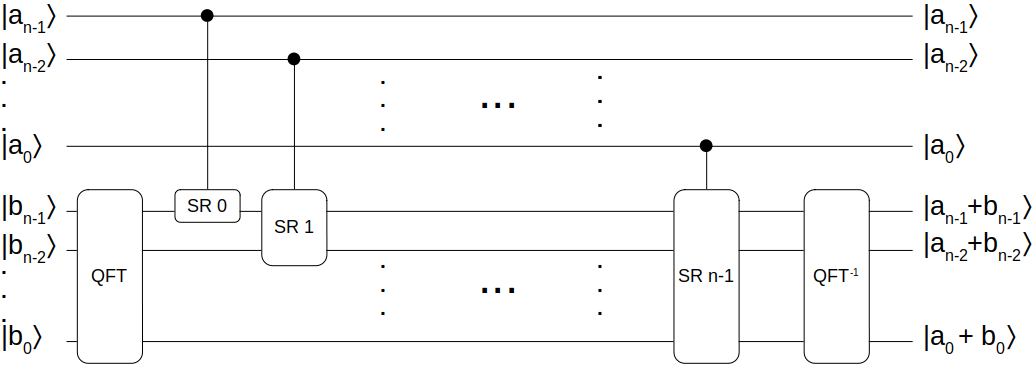
\includegraphics[width=1\textwidth]{qft-adder.png}
  \footnotesize
  \Qcircuit @C=0.25em @R=0.4em {
    \lstick{\qket{x_{n-1}}} & \multigate{4}{\texttt{$x-2^{I-i} n$}} & \multigate{4}{ \texttt{QFT}^{-1}\;N } & \ctrl{9} & \multigate{4}{ \texttt{QFT}\;N } & \multigate{4}{\texttt{$x+2^{I-i} n$}} & \qw & \qw & \qw \\
    \lstick{\qket{x_{n-2}}} &  \ghost{\texttt{$x-2^{I-i} n$}} & \ghost{ \texttt{QFT}^{-1}\;N } & \qw & \ghost{ \texttt{QFT}\;N } & \ghost{\texttt{$x+2^{I-i} n$}} & \qw & \qw & \qw \\
    \lstick{\vdots} & & & & & & & &  \rstick{\vdots} \\
    \lstick{} & &  & & & & & & \\
    \lstick{\qket{x_0}} & \ghost{\texttt{$x-2^{I-i} n$}}  & \ghost{ \texttt{QFT}^{-1}\;N } & \qw & \ghost{ \texttt{QFT}\;N } & \ghost{\texttt{$x+2^{I-i} n$}} & \qw & \qw & \qw  \\
\lstick{} & & & & & & & & &\\
    \lstick{\ket{b_{n-1}}} & \qw & \qw & \qw  & \qw & \qw & \qw & \qw & \qw   \\
    \lstick{\vdots} & & & & \dots &  & &   \\
    \lstick{} & & & & &  & & &   \\
    \lstick{\ket{b_{1}}} & \qw & \qw  &  \targ  & \qw & \ctrl{-5} & \qw & \targ & \qw   \\
    \lstick{\vdots} & & & & & & & &  \rstick{\vdots} \\
    \lstick{} & & & & & & & & &  \\
    \lstick{\ket{b_0}} & \qw & \qw & \qw & \qw & \qw & \qw & \qw & \qw  
    }
\subcaption{QFT-based}
\end{minipage} 
\\\\
\begin{minipage}{.7\textwidth}
% 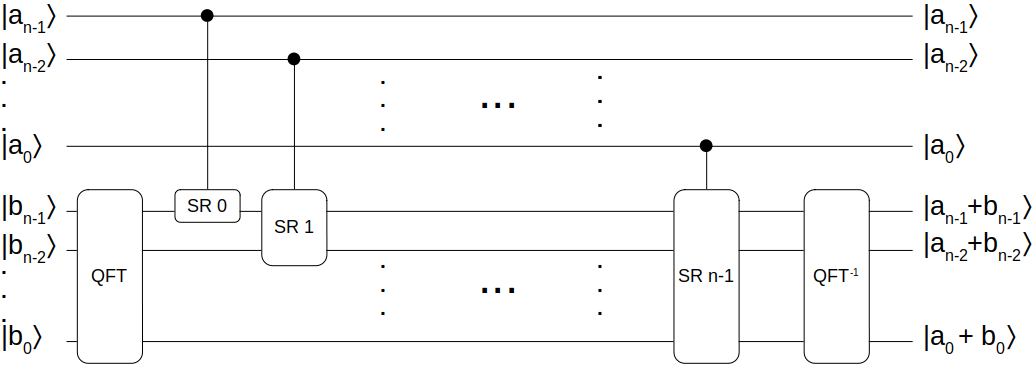
\includegraphics[width=1\textwidth]{qft-adder.png}
  \footnotesize
  \Qcircuit @C=0.25em @R=0.4em {
    \lstick{\qket{x_{n-1}}} & \multigate{4}{\texttt{$x-2^{I-i} n$}} & \multigate{4}{ \texttt{QFT}^{-1}\;(N-i) } & \qw & \qswap & \qw & \multigate{4}{ \texttt{RSH} } & \multigate{4}{ \texttt{QFT}\;(N-i-1) } & \multigate{4}{x+(2^{I-i} n \!\mod 2^{I-i-1})} & \qw & \qw & \qw & \qw  \\
    \lstick{\qket{x_{n-2}}} &  \ghost{\texttt{$x-2^{I-i} n$}} & \ghost{ \texttt{QFT}^{-1}\;(N-i) } & \qw & \qw \qwx &\qw & \ghost{ \texttt{RSH} } & \ghost{ \texttt{QFT}\;(N-i-1) } & \ghost{x+(2^{I-i} n \!\mod 2^{I-i-1})} & \qw & \qw & \qw & \qw \\
    \lstick{\vdots} & & & & \qwx & & & & & & & &  \rstick{\vdots} \\
    \lstick{} & &  & & \qwx & & & & & & & &  \\
    \lstick{\qket{x_0}} & \ghost{\texttt{$x-2^{I-i} n$}}  & \ghost{ \texttt{QFT}^{-1}\;(N-i) } & \qw & \qw \qwx & \qw & \ghost{\texttt{RSH}} & \ghost{ \texttt{QFT}\;(N-i-1) } & \ghost{x+(2^{I-i} n \!\mod 2^{I-i-1})} & \qw & \qw & \qw & \qw  \\
    \lstick{} & & & & \qwx & & & & & & & & & \\
    \lstick{\ket{b_{n-1}}} & \qw & \qw & \qw & \qw \qwx & \qw & \qw & \qw & \qw & \qw & \qw & \qw & \qw \\
    \lstick{\vdots} & & & & \qwx & & & \dots &  & & & & \\
    \lstick{} & & & & \qwx & & & & & & & & & \\
    \lstick{\ket{b_{1}}} & \qw & \qw  & \qw &  \qswap \qwx & \qw & \qw & \qw & \ctrl{-5} & \qw & \targ & \qw & \qw \\
    \lstick{\vdots} & & & & & & & & &&  & &  \rstick{\vdots} \\
    \lstick{} & & & & & & & & && & &  \\
    \lstick{\ket{b_0}} & \qw & \qw & \qw & \qw & \qw & \qw & \qw & \qw & \qw & \qw & \qw  & \qw 
    }
\subcaption{AQFT-based (addition and subtraction are approximate)}
\end{minipage} 
\end{tabular}
}
\caption{One step of the QFT/AQFT division/modulo circuit}
\label{fig:qft-moder}
\end{figure*}

\ignore{
\begin{figure*}[t]
\centering

\begin{coq}
Fixpoint appx_moder' i (n:nat) (b:nat) (x ex:var) (M:nat -> bool) := 
     match i with 0 =>  (SKIP (x,0))
           | S j => appx_compare_half3 x n b (ex,j) M ;  Rshift x;
                     QFT x b; (CU (ex,j) ((appx_adder x n b M)));
                      (X (ex,j)); 
                       appx_moder' j n (b+1) x ex (cut_n (div_two_spec M) n)
     end.
\end{coq}
\caption{Approximate QFT Modulo Operation (Core of Addition/Subtraction in \Cref{fig:circuit-add-sub})}
\label{fig:qft-moder}
\end{figure*}
}

Even though the approximate adder is not particularly useful for addition, there are still cases where it can be useful as a subcomponent. 
For example, the modulo/division circuit relies on an addition subcomponent, but does not need every bit to be correctly added.

\Cref{fig:qft-moder}(a) shows one step of an $N$-bit QFT-based modulo circuit that computes $x\!\!\mod n$ for constant $n$.
The algorithm runs for $I+1$ iterations, where $2^{N-1} \le 2^I n <2^N$, with the iteration counter $i$ increasing from 0 to $I$ (inclusive).
In each iteration, the circuit in \Cref{fig:qft-moder}(a) computes $x-2^{I-i} n$ and uses the result's most significant bit (MSB) to check whether $x < 2^{N-1-i}$.
If the MSB is $0$, then $x \ge 2^{N-1-i}$ and the circuit continues to next iteration; otherwise, it adds $2^{I-i} n$ to the result and continues.

We can improve the resource usage of the circuit in \Cref{fig:qft-moder}(a) by replacing the addition, subtraction, and QFT components with approximate versions, as shown in \Cref{fig:qft-moder}(b).
At the start of each iteration, $x < 2^{N-i}$, so it is safe to replace components with versions that will perform the intended operation on the lowest $(N-i)$ bits.
The circuit in \Cref{fig:qft-moder}(b) begins by subtracting the top $(N-i)$ bits, and then converts $x$ back to the \texttt{Nor} basis using an $(N-i)$-bit precision QFT\@.
It then swaps the MSB with an ancilla, guaranteeing that the MSB is 0. 
Next, it uses a \texttt{Rshift} to move the cleaned MSB to become the lowest significant bit (effectively, multiplying $x$ by 2) and uses a $(N-i-1)$-bit precision QFT to convert back to the \texttt{Phi} basis.
Finally, it conditionally adds back the top $(N-i-1)$ bit of the value $(2^{I-i} n \!\mod 2^{I-i-1})$, ignoring the original MSB.

The result is a division/modulo circuit that uses approximate components, but, as our testing assures, is exactly correct.
\Cref{fig:approx-results}(b) shows the required resources for varying numbers of iterations.
Compared to QFT-based circuit,
for a single iteration, the approximation provides a 4.5\% savings, and the saving increases with more iterations.
For $n = 1$, we need 16 iterations. In this case, the AQFT-based division/modulo circuit uses 61.1\% fewer gates than the QFT-based implementation.
If we compare the AQFT-based division/modulo circuit with the Toffoli-based one, the result is more significant. For 16 iterations, the AQFT-based division/modulo circuit uses 79.3\% fewer gates than the Toffoli-based implementation.

\section{Evaluation: \vqimp Oracles and Partial Evaluation}
\label{sec:partial-eval}

The prior section considered arithmetic operators implemented in
\oqasm. They are building blocks for operators we have programmed using
\vqimp, which include sine, 
arcsine, cosine, arccosine, and exponentiation on fixed-precision
numbers. We used \vqimp's source semantics to test each operator's
correctness.
These operators are useful in near-term applications; e.g., the
arcsine and sine functions are sub-components to repair the phase
values in constructing Hamiltonian simulations~\cite{feynman1982simulating} by the quantum walk
algorithm~\cite{Childs_2009}. 

As discussed in \Cref{sec:qimp}, one of the key features of \vqimp is \emph{partial evaluation} during compilation to \vqir.
The simplest optimization similar to partial evaluation happens for a
binary operation $x := x\odot y$, where $y$ is a constant value. 
\Cref{fig:circ-evaluation} hints at the power of partial evaluation for this case---all constant operations (marked ``const'') generate circuits with significantly fewer qubits and gates.
Languages like Quipper take advantage of this by producing special circuits for operations that use classically-known constant parameters.

Partial evaluation takes this one step further, pre-evaluating as much of the circuit as possible.
For example, consider the fixed precision operation $\frac{x*y}{M}$ where
$M$ is constant and a natural number, and $x$ and $y$ are two fixed precision numbers that may be constants.
This is a common pattern, appearing in many quantum oracles (recall the $\frac{8^n*x}{n!}$ in the Taylor series decomposition of sine). 
In Quipper, this is expression compiled to ${r_1}\texttt{ = }{\frac{x}{M}}; {r_2}\texttt{ = }{r1*y}$.
%
The \vqimp compiler produces different outputs depending on whether $x$ and $y$ are constants. If they both are constant, \vqimp simply assigns the result of computing $\frac{x*y}{M}$ to a quantum variable. If $x$ is a constant, but $y$ is not, \vqimp evaluates $\frac{x}{M}$ classically, assigns the value to $r_1$, and evaluates $r_2$ using a constant multiplication circuit. If they are both quantum variables, \vqimp generates a circuit to evaluate the division first and then the multiplication.

In \Cref{fig:self-data}~(a) we show the size of the circuit generated for $\frac{x*y}{M}$ where zero, one, or both variables are classically known. 
It is clear that more classical variables in a program lead to a more efficient output circuit.
If $x$ and $y$ are both constants, then only a constant assignment circuit is needed, which is a series of \texttt{X} gates. 
Even if only one variable is constant, it may lead to substantial savings: In this example, if $x$ is constant, the compiler can avoid the division circuit and use a constant multiplier instead of a general multiplier.
These savings quickly add up: \Cref{fig:self-data}~(b) shows the qubit size difference between our implementation of sine and Quippers'. Both the TOFF and QFT-based circuits use fewer than $7\%$ of the qubits used by Quipper's sine implementation.
\footnote{\vqimp also benefits from its representation of fixed-precision numbers (\Cref{sec:qimp}), which is more restrictive than Quipper's. Our representation of fixed-precision numbers reduces the qubit usage of the sine function by half, so about half of the qubit savings can be attributed to this.}

\begin{figure}[t]
{\small
\begin{subfigure}[b]{.6\textwidth}
\centering
\begin{tabular}{| l | c | c |}
\hline
                     & \# qubits  & \# gates   \\
                     \hline
OQIMP ($x$, $y$ const) & 16 & 16\\
OQIMP TOFF ($x$ const) & 33 & $1739 \pm 376$ \\
OQIMP QFT ($x$ const) & 16 & $1372 \pm 26$ \\
OQIMP TOFF & 33 & 61470   \\
OQIMP QFT & 32  & 25609  \\
\hline                           
\end{tabular}
  \subcaption{
Fixed-precision circuits for $\frac{x*y}{M}$ with $M=5$ (16 bits)
}
\end{subfigure}
\hfill
\begin{subfigure}[b]{.35\textwidth}
\centering
\begin{tabular}{| l | c|}
\hline
                     & \# qubits   \\
                     \hline
OQIMP TOFF & 418   \\
OQIMP QFT & 384  \\
Quipper & 6142  \\
\hline                           
\end{tabular}
  \subcaption{
Sine circuits (64 bits)}
\end{subfigure}
}
\caption{Effects of partial evaluation}
\label{fig:self-data}
\end{figure}

\section{Case Study: Grover's Search}
\label{sec:grovers}

Here we present a case study of integrating an oracle implemented with \name into a full quantum algorithm, Grover's search algorithm, implemented and verified in \sqir.

Grover's search algorithm \cite{grover1996,grover1997}, described in \Cref{sec:background}, has implications for cryptography, in part because it can be used to find collisions in cryptographic hash functions \cite{grover-hash}. Thus, the emergence of quantum computers may require lengthening hash function outputs.

We have used \vqimp to implement the ChaCha20 stream cipher \cite{chacha} as an oracle for Grover's search algorithm. 
%\name proved especially useful for this task, as \vqimp contains many of the operations commonly used by cryptographic hash functions, and any oracles were written can be efficiently tested on a classical machine.
%
This cipher computes a hash of a 256-bit key, a 64-bit message number, and a 64-bit block number, and it is actively being used in the TLS protocol \cite{rfc7905,rfc8446}.
The procedure consists of twenty cipher rounds, most easily implemented when segmented into quarter-round and double-round subroutines. 
The only operations used are bitwise \textsc{xor}, bit rotations, and addition modulo $2^{32}$, all of which are included in \vqimp; the implementation is given in \Cref{fig:chacha-qr}.

To test our oracle implementation, we wrote our specification as a Coq function on bitstrings.
We then defined correspondence between these bitstrings and program states in \vqir semantics and conjectured that for any inputs, the semantics of our compiled oracle matches the corresponding outputs from our specification function.
Using random testing (\Cref{sec:rand-testing}),
we individually tested the quarter-round and double-round subroutines as well as the whole twenty-round cipher, performing a sort of unit testing.
We also tested the oracle for the boolean-valued function that checks whether the ChaCha20 output matches a known bitstring rather than producing the output directly.
This oracle can be compiled to \sqir using our verified compiler, and then the compiled oracle can be used by Grover's algorithm to invert the ChaCha20 function and find collisions.
Grover's algorithm was previously implemented and verified in \sqir \cite{PQPC}, and we have modified this implementation and proof to allow for oracles with ancillae like the ones generated by our compiler; thus, our successful QuickChick tests combined with the previously proved theorems for Grover's algorithm provide confidence that we can find Chacha20's hash collisions in a certain probability through Grover's algorithm.

\begin{figure}[t]
\[\footnotesize
\begin{array}{l}
Q\;\tnat[4]\;qr(Q\;\tnat\;x_1,Q\;\tnat\;x_2,Q\;\tnat\;x_3,Q\;\tnat\;x_4)\;\{
\\
\quad{x_1}\texttt{ += }{x_2};\; {x_4}{\; \oplus\texttt{= } }{x_1};\; x_4\,\texttt{<{}<{}<=}\,16;\\
\quad{x_3}\texttt{ += }{x_4};\; {x_2}{\; \oplus\texttt{= } }{x_3};\; x_4\,\texttt{<{}<{}<=}\,12;\\
\quad{x_1}\texttt{ += }{x_2};\; {x_2}{\; \oplus\texttt{= } }{x_1};\; x_4\,\texttt{<{}<{}<=}\,8;\\
\quad{x_3}\texttt{ += }{x_4};\; {x_2}{\; \oplus\texttt{= } }{x_3};\; x_4\,\texttt{<{}<{}<=}\,7\\
\quad\texttt{return}\;[x_1,x_2,x_3,x_4];\\
\}\\\\
\texttt{void}\;chacha20(Q\;\tnat[16]\;x)\;\{
\\
\quad\texttt{for}(C\;\tnat\;i=20;\;i>0;\;i \texttt{ -= } 2)\;\{\\
\qquad [x[0], x[4], x[8], x[12]] = qr(x[0], x[4], x[8], x[12]);\\
\qquad [x[1], x[5], x[9], x[13]] = qr(x[1], x[5], x[9], x[13]);\\
\qquad [x[2], x[6], x[10], x[14]] = qr(x[2], x[6], x[10], x[14]);\\
\qquad [x[3], x[7], x[11], x[15]] = qr(x[3], x[7], x[11], x[15]);\\
\qquad [x[0], x[5], x[10], x[15]] = qr(x[0], x[5], x[10], x[15]);\\
\qquad [x[1], x[6], x[11], x[12]] = qr(x[1], x[6], x[11], x[12]);\\
\qquad [x[2], x[7], x[8], x[13]] = qr(x[2], x[7], x[8], x[13]);\\
\qquad [x[3], x[4], x[9], x[14]] = qr(x[3], x[4], x[9], x[14]);\\
\quad\}\\
\}
\end{array}
\]
\caption{ChaCha20 implementation in \vqimp}
\label{fig:chacha-qr}
\end{figure}
